% Author: Izaak Neutelings (November 2020)
\documentclass[border=3pt,tikz]{standalone}
\usepackage{physics}
\usepackage{tikz}
\usepackage[outline]{contour} % glow around text
\usetikzlibrary{patterns,decorations.pathmorphing}
\usetikzlibrary{decorations.markings}
\usetikzlibrary{arrows.meta}
\usetikzlibrary{calc}
\tikzset{>=latex}
\contourlength{1.1pt}

\colorlet{mydarkblue}{blue!40!black}
\colorlet{myblue}{blue!70!black}
\colorlet{myred}{red!65!black}
\colorlet{myorange}{orange!90!black!90}
\colorlet{vcol}{green!45!black}
\colorlet{watercol}{blue!80!cyan!10!white}
\colorlet{darkwatercol}{blue!80!cyan!80!black!30!white}
\colorlet{metalcol}{blue!25!black!30!white}
\tikzstyle{piston}=[blue!50!black,top color=blue!30,bottom color=blue!50,middle color=blue!20,shading angle=0]
\tikzstyle{water}=[draw=mydarkblue,rounded corners=0.1,top color=watercol!90,bottom color=watercol!90!black,middle color=watercol!50,shading angle=20]
\tikzstyle{horizontal water}=[water,top color=watercol!90!black!90,bottom color=watercol!90!black!90,middle color=watercol!80,shading angle=0]
\tikzstyle{metal}=[draw=metalcol!10!black,rounded corners=0.1,top color=metalcol,bottom color=metalcol!80!black,shading angle=10]
\tikzstyle{vvec}=[->,very thick,vcol,line cap=round]
\tikzstyle{force}=[->,myred,very thick,line cap=round]
\tikzstyle{width}=[{Latex[length=4,width=3]}-{Latex[length=4,width=3]}]
\def\tick#1#2{\draw[thick] (#1)++(#2:0.12) --++ (#2-180:0.24)}

\begin{document}


% LAMINAR FLOW LAYERS
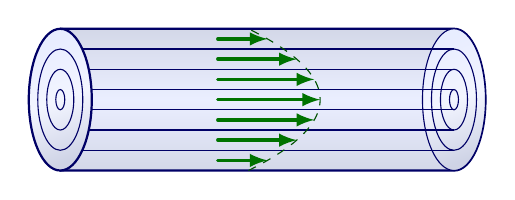
\begin{tikzpicture}
  \def\L{5.0}   % total length
  \def\Rx{0.40} % big pipe vertical radius right
  \def\Ry{0.90} % big pipe vertical radius right
  \def\v{1.3}   % velocity magnitude
  \def\N{3}     % velocity magnitude
  
  % WATER
  \draw[horizontal water,thick]
    (0,\Ry) -- (0,-\Ry)  coordinate (A1) --++ (\L,0) arc(-90:90:{\Rx} and \Ry) -- cycle;
  \draw[water]
    (\L,0) ellipse({\Rx} and \Ry);
  
  \draw[water]
    (0,0) ellipse({\Rx} and \Ry);
  %\draw[horizontal water,line width=0.1] %draw=none
  %  (0,-\Ry) rectangle (\L,\Ry);
  \foreach \i [evaluate={\x=(\i-0.5)/(\N+0.5)}] in {1,...,\N}{
    \draw[mydarkblue] %,line width=0.05
      (0,0) ellipse({\x*\Rx} and \x*\Ry)
      (\L,0) ellipse({\x*\Rx} and \x*\Ry);
    \draw[mydarkblue] %,dashed]  %,line width=0.05
      (0, \x*\Ry) --++ (\L,0)
      (0,-\x*\Ry) --++ (\L,0); %arc(90:-90:{\x*\Rx} and \x*\Ry) --++ (-\L,0);
  }
  %\draw[horizontal water,draw=none]
  %  (0,{-\N/(\N+1)*\Ry}) rectangle (\L,{\N/(\N+1)*\Ry});
  \draw[water,thick]
    (0,0) ellipse({\Rx} and \Ry);
  \foreach \i [evaluate={\x=(\i-0.5)/(\N+0.5)}] in {1,...,\N}{
    \draw[mydarkblue] (0,0) ellipse({\x*\Rx} and \x*\Ry);
  }
  %\draw[mydarkblue,thick]
  %  (0,\Ry) arc(90:-90:{\Rx} and \Ry) coordinate (A1) --++ (\L,0) arc(-90:90:{\Rx} and \Ry) -- cycle;
  \draw[vcol!70!black,dashed,samples=100,smooth,variable=\y,domain=-1:1]
    plot({0.4*\L+\v*(1-0.7*\y*\y)},\y*\Ry);
  \draw[vvec] (0.4*\L,0) --++ (\v,0);
  \foreach \i [evaluate={\y=(\i)/(\N+0.5); \vy=\v*(1-0.7*\y^2);}] in {1,...,\N}{
    \draw[vvec] (0.4*\L, \y*\Ry) --++ (\vy,0);
    \draw[vvec] (0.4*\L,-\y*\Ry) --++ (\vy,0);
  }
  
\end{tikzpicture}


% PRESSURE
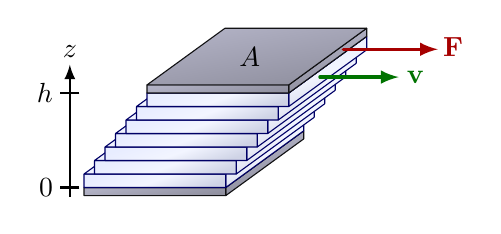
\begin{tikzpicture}[x={(1cm,0)},y={(0.55cm,0.40cm)},z={(0,1cm)}]
  \def\L{1.8}   % cube side
  \def\H{1.2}   % total height
  \def\d{0.8}   % total distance
  \def\N{7}     % number of layers
  \def\t{\H/\N} % layer thickness
  %\draw[dark water] (0,0,0) -- (\L,0,0) -- (\L,\L,0) -- ( 0,\L,0) -- cycle;
  \def\layer#1#2#3#4{
    \draw[#1] (#2+\L,0,#3) --++ (0,\L,0) --++ (0,0,-#4) --++ (0,-\L,0) -- cycle;
    \draw[#1] (#2,0,#3) --++ (\L,0,0) --++ (0,0,-#4) --++ (-\L,0,0) -- cycle;
    \draw[#1] (#2,0,#3) --++ (\L,0,0) --++ (0,\L,0) --++ (-\L,0,0) -- cycle;
  }
  
  \layer{metal}{0}{0}{0.6*\t}
  \foreach \i [evaluate={\x=(\i-1)*\d/(\N-1); \ya=\i*\H/\N; \yb=(\i-1)*\H/\N;}] in {1,...,\N}{
    \layer{water}{\x}{\ya}{\t}
  }
  \layer{metal}{\d}{\H+0.6*\t}{0.6*\t}
  \draw[force] (\L+\d,0.7*\L,\H+0.3*\t) --++ (1.2,0,0) node[above=1,right=-2] {$\vb{F}$};
  \draw[vvec] (\L+\d,0.4*\L,\H-0.5*\t) --++ (1,0,0) node[below=0,right=-1] {$\vb{v}$};
  \node at (\d+0.45*\L,0.5*\L,\H+0.6*\t) {$A$};
  %\draw[width] (0.06*\L,0,0) --++ (0,0,\H) node[midway,fill=white,inner sep=0.5] {$h$};
  \draw[->,thick]
    (-0.1*\L,0,-0.1*\H) --++ (0,0,1.4*\H) node[above=-1] {$z$};
  \tick{-0.1*\L,0,0}{0} node[left=-1] {0};
  \tick{-0.1*\L,0,\H}{0} node[left=-1] {$h$};
  
\end{tikzpicture}


% LAMINAR FLOW around object
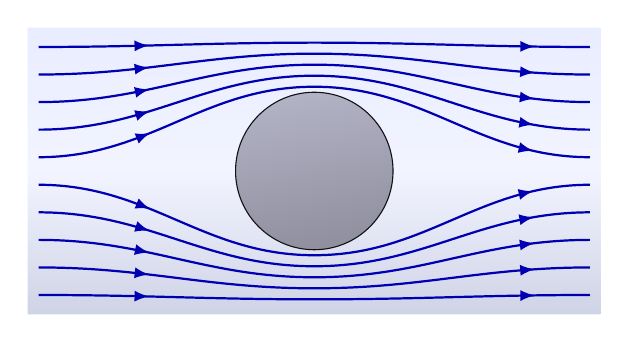
\begin{tikzpicture}
  \def\W{7.0}   % total length
  \def\H{3.5}   % total height
  \def\R{1.0}   % total distance
  \def\N{5}     % number of layers
  \def\t{\H/\N} % layer thickness
  \draw[water,shading angle=0,draw=none]
    (-0.52*\W,-0.52*\H) rectangle (0.52*\W,0.52*\H);
  \draw[metal]
    (0,0) circle(\R);
  \foreach \s in {-1,1}{
    \foreach \i [evaluate={\fy=\s*(\i-0.5)/\N; \y=\fy*0.5*\H;}] in {1,...,\N}{
      \draw[myblue,thick,postaction={decorate},decoration={markings,
        mark=at position {0.2} with {\arrow{latex}},mark=at position 0.9 with {\arrow{latex}}}]
        (-\W/2,\y) to[out=0,in=180] (0,\s*\R+0.7*\fy) to[out=0,in=180] (\W/2,\y);
    }
  }
\end{tikzpicture}


% TURBULENCE around object
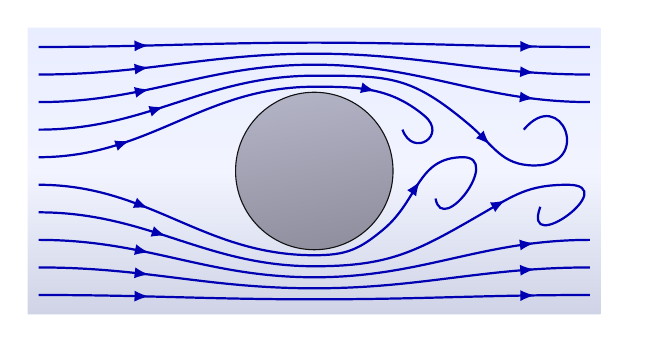
\begin{tikzpicture}
  \def\W{7.0}   % total length
  \def\H{3.5}   % total height
  \def\R{1.0}   % total distance
  \def\N{5}     % number of layers
  \def\t{\H/\N} % layer thickness
  \draw[water,shading angle=0,draw=none]
    (-0.52*\W,-0.52*\H) rectangle (0.52*\W,0.52*\H);
  \draw[metal]
    (0,0) circle(\R);
  \foreach \s in {-1,1}{
    \foreach \i [evaluate={\fy=\s*(\i-0.5)/\N; \y=\fy*0.5*\H;}] in {3,...,\N}{
      \draw[myblue,thick,postaction={decorate},decoration={markings,
        mark=at position {0.2} with {\arrow{latex}},mark=at position 0.9 with {\arrow{latex}}}]
        (-\W/2,\y) to[out=0,in=180] (0,\s*\R+0.7*\fy) to[out=0,in=180] (\W/2,\y);
    }
  }
  
  %\def\p{node[circle,fill=red,inner sep=0.9] {}} % probe dot
  \draw[myblue,thick,postaction={decorate},decoration={markings,
    mark=at position {0.2} with {\arrow{latex}},mark=at position 0.75 with {\arrow{latex}}}]
    (-\W/2,{1.5/\N*0.5*\H}) to[out=0,in=180] (0,{\R+0.7*1.5/\N}) to[out=0,in=140,looseness=1.2]
    (0.28*\W,0.17*\H) to[out=-40,in=180,looseness=1.1] (0.40*\W,0.02*\H) to[out=0,in=50,looseness=4]
    (0.38*\W,0.15*\H);
  \draw[myblue,thick,postaction={decorate},decoration={markings,
    mark=at position {0.2} with {\arrow{latex}},mark=at position 0.75 with {\arrow{latex}}}]
    (-\W/2,{0.5/\N*0.5*\H}) to[out=0,in=180] (0,{\R+0.7*0.5/\N}) to[out=0,in=140,looseness=1.0]
    (0.20*\W,0.20*\H) to[out=-40,in=-70,looseness=3] (0.16*\W,0.15*\H);
  \draw[myblue,thick,postaction={decorate},decoration={markings,
    mark=at position {0.2} with {\arrow{latex}},mark=at position 0.75 with {\arrow{latex}}}]
    (-\W/2,{-0.5/\N*0.5*\H}) to[out=0,in=180] (0,{-\R-0.7*0.5/\N}) to[out=0,in=-140,looseness=1.1]
    (-40:1.15*\R) to[out=40,in=180,looseness=1.1] (0.27*\W,0.05*\H) to[out=0,in=-80,looseness=2]
    (0.22*\W,-0.10*\H);
  \draw[myblue,thick,postaction={decorate},decoration={markings,
    mark=at position {0.2} with {\arrow{latex}},mark=at position 0.75 with {\arrow{latex}}}]
    (-\W/2,{-1.5/\N*0.5*\H}) to[out=0,in=180] (0,{-\R-0.7*1.5/\N}) to[out=0,in=-150,looseness=1.1]
    (0.30*\W,-0.16*\H) to[out=30,in=180,looseness=1.1] (0.46*\W,-0.05*\H) to[out=0,in=-110,looseness=4]
    (0.41*\W,-0.13*\H);
  
\end{tikzpicture}


% TURBULENCE - REYNOLDS
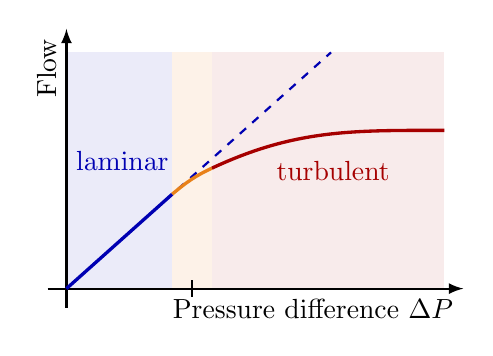
\begin{tikzpicture}
  \def\xmax{4.8}
  \def\ymax{3.0}
  \def\xa{0.40*0.7*\xmax}
  \def\xb{0.55*0.7*\xmax}
  \fill[myblue!8] (0,0) rectangle (\xa,\ymax);
  \fill[myorange!10] (\xa,0) rectangle (\xb,\ymax);
  \fill[myred!8] (\xb,0) rectangle (\xmax,\ymax);
  \draw[->,thick] (-0.05*\xmax,0) -- (1.05*\xmax,0) node[below left=0] {Pressure difference $\Delta P$};
  \draw[->,thick] (0,-0.05*\xmax) -- (0,1.10*\ymax) node[above left=0,rotate=90] {Flow};
  \draw[thick] ({(\xa+\xb)/2},0.035*\ymax) --++ (0,-0.07*\ymax);
  \draw[thick,myblue,dashed] (0,0) -- (0.7*\xmax,\ymax);
  \draw[very thick,myblue] (0,0) -- (\xa,0.40*\ymax) coordinate (T1);
  \draw[very thick,myorange] (T1) to[out=40,in=-155] (\xb,0.51*\ymax) coordinate (T2);
  \draw[very thick,myred] (T2) to[out=25,in=180] (\xmax,0.67*\ymax);
  \node[right,myblue] at (0,0.54*\ymax) {laminar};
  \node[right,myred] at (0.53*\xmax,0.50*\ymax) {turbulent};
  %\draw[dashed] ({(\xa+\xb)/2},0) --++ (0,\ymax) node[above] {$\mathrm{Re}\sim2300$};
\end{tikzpicture}


\end{document}
